\section{Results}
\label{sec:results}

This section first compares the proposed RF300-F0.7 configuration with the full-feature RF300-F1.0 baseline on the original benchmark and on the independent EETAC dataset. It then analyzes the subspace ratio itself (density dependence and selection), compares the configuration with literature ensembles, and reports computational cost and uncertainty calibration.

% ============================================================
\subsection{Original Benchmark Localization Accuracy}
\label{subsec:original_results}

Table~\ref{tab:original_accuracy} reports the localization results on the official Building, Office, and Apartment test sets, which are RP-disjoint from the training sets.

\begin{table*}[!t]
\centering
\caption{Point-localization performance on the original hybrid RTT--RSS benchmark (official RP-disjoint test sets). The paper-compatible metric is defined in Eq.~\eqref{eq:paper_metric}. 95\% CI: paired cluster bootstrap over test RPs (1000 replicates) of the F0.7$-$F1.0 difference in the paper-compatible metric; an interval excluding zero indicates a reliable improvement.}
\label{tab:original_accuracy}
\footnotesize
\setlength{\tabcolsep}{4pt}
\begin{tabular}{lccccccccc}
\toprule
 & \multicolumn{5}{c}{Paper-compatible metric (m)} & \multicolumn{2}{c}{2D RMSE (m)} & \multicolumn{2}{c}{$P_{90}$ (m)} \\
\cmidrule(lr){2-6}\cmidrule(lr){7-8}\cmidrule(lr){9-10}
Dataset & Published & F1.0 & F0.7 & Impr. (\%) & 95\% CI of diff. & F1.0 & F0.7 & F1.0 & F0.7 \\
\midrule
Building & 0.600 & 0.599 & \textbf{0.513} & 14.32 & [-0.109, -0.064] & 0.851 & \textbf{0.732} & 1.216 & \textbf{1.079} \\
Office & 0.380 & 0.370 & \textbf{0.343} & 7.05 & [-0.048, -0.008] & 0.523 & \textbf{0.486} & 0.827 & \textbf{0.758} \\
Apartment & 0.590 & 0.600 & \textbf{0.569} & 5.14 & [-0.107, +0.057] & 0.867 & \textbf{0.821} & \textbf{1.163} & 1.235 \\
\bottomrule
\end{tabular}
\end{table*}


The reproduced RF300-F1.0 results closely match the published hybrid RTT--RSS values: $0.599$ versus $0.600$~m for Building, $0.370$ versus $0.380$~m for Office, and $0.600$ versus $0.590$~m for Apartment. The reproduction also shows that the published values correspond to the mean of the per-coordinate RMSEs: the true two-dimensional RMSE of the same models is $0.851$, $0.523$, and $0.867$~m.

RF300-F0.7 reduces the paper-compatible error from $0.599$ to $0.513$~m in Building ($14.32\%$), from $0.370$ to $0.343$~m in Office ($7.05\%$), and from $0.600$ to $0.569$~m in Apartment ($5.14\%$). The 2D RMSE decreases from $0.851$ to $0.732$~m, from $0.523$ to $0.486$~m, and from $0.867$ to $0.821$~m, respectively. The paired cluster bootstrap over test RPs gives 95\% confidence intervals of $[-0.109,-0.064]$~m for Building and $[-0.048,-0.008]$~m for Office, so these improvements are reliable. For Apartment, which has only 29 test RPs, the interval $[-0.107,+0.057]$~m includes zero: the official test alone does not establish the Apartment improvement, which is instead supported by the grouped-CV, seed, and density analyses below.

The $P_{90}$ error decreases from $1.216$ to $1.079$~m in Building and from $0.827$ to $0.758$~m in Office. In Apartment, the average error decreases but $P_{90}$ increases from $1.163$ to $1.235$~m, so the configuration improves the central part of the error distribution there without improving its upper tail. The empirical error distributions are shown in the supplementary material (Fig.~S1).

These values come from a single forest seed. Table~\ref{tab:robustness} repeats the comparison with ten seeds: $\rho=0.7$ has the lower error in all 30 seed--environment pairs, with mean improvements of $14.4\pm0.7\%$ (Building), $9.2\pm1.5\%$ (Office), and $5.2\pm1.2\%$ (Apartment). The Apartment $P_{90}$ increase, by contrast, is systematic: it occurs in all ten seeds. The seed variability is therefore small compared with the Building and Office gains, whereas the Apartment result remains a small mean improvement with a heavier upper tail.

\begin{table*}[!t]
\centering
\caption{Robustness of the comparison $\rho=0.7$ versus $\rho=1$ over ten seeds (0--9). Improvement: relative error reduction (paper-compatible metric for the benchmark, 2D RMSE for EETAC), mean $\pm$ standard deviation over seeds. Wins: seeds in which $\rho=0.7$ has the lower error (or lower $P_{90}$). CI: 95\% paired RP-clustered bootstrap interval of the 2D RMSE difference ($\rho=0.7$ minus $\rho=1$, m) for seed 0; for the official tests, see Table~\ref{tab:original_accuracy}.}
\label{tab:robustness}
\footnotesize
\setlength{\tabcolsep}{4pt}
\begin{tabular}{llcccc}
\toprule
Dataset & Protocol & Improvement (\%) & Wins (error) & Wins ($P_{90}$) & 95\% CI of difference (m) \\
\midrule
Building & official test & 14.4 $\pm$ 0.7 & 10/10 & 10/10 & -- \\
Apartment & official test & 5.2 $\pm$ 1.2 & 10/10 & 0/10 & -- \\
Office & official test & 9.2 $\pm$ 1.5 & 10/10 & 10/10 & -- \\
\midrule
EETAC Medium & sample-level CV & 13.7 $\pm$ 1.3 & 10/10 & -- & [-0.086, -0.017] \\
 & RP-grouped CV & 13.8 $\pm$ 0.5 & 10/10 & -- & [-0.575, -0.213] \\
 & Day~1$\rightarrow$Day~2 & 5.6 $\pm$ 1.3 & 10/10 & -- & [-0.158, -0.031] \\
 & Day~2$\rightarrow$Day~1 & 20.4 $\pm$ 1.7 & 10/10 & -- & [-0.603, -0.001] \\
EETAC High & sample-level CV & 13.7 $\pm$ 1.1 & 10/10 & -- & [-0.080, -0.021] \\
 & RP-grouped CV & 13.2 $\pm$ 0.3 & 10/10 & -- & [-0.551, -0.185] \\
 & Day~1$\rightarrow$Day~2 & 0.2 $\pm$ 2.3 & 4/10 & -- & [-0.151, +0.036] \\
 & Day~2$\rightarrow$Day~1 & 13.2 $\pm$ 1.4 & 10/10 & -- & [-0.427, +0.008] \\
\bottomrule
\end{tabular}
\end{table*}


% ============================================================
\subsection{RP-Grouped Cross-Validation}
\label{subsec:grouped_cv_results}

The official test is a single split. Five-fold RP-grouped CV on the training RPs (Table~\ref{tab:grouped_cv}) provides a second estimate that, like the official test, evaluates unseen locations, but trains each fold model on only about $80\%$ of the training RPs.

\begin{table*}[!t]
\centering
\caption{Five-fold RP-grouped validation on the official training RPs of the original benchmark. All metrics are computed on the pooled out-of-fold predictions. Each fold model is trained on about $80\%$ of the training RPs, i.e., on a sparser radio map than the official-test models.}
\label{tab:grouped_cv}
\footnotesize
\setlength{\tabcolsep}{4.5pt}
\begin{tabular}{lccccccccc}
\toprule
 & \multicolumn{3}{c}{Paper-compatible metric (m)} & \multicolumn{2}{c}{2D RMSE (m)} & \multicolumn{2}{c}{$P_{90}$ (m)} & \multicolumn{2}{c}{$P_{95}$ (m)} \\
\cmidrule(lr){2-4}\cmidrule(lr){5-6}\cmidrule(lr){7-8}\cmidrule(lr){9-10}
Dataset & F1.0 & F0.7 & Impr. (\%) & F1.0 & F0.7 & F1.0 & F0.7 & F1.0 & F0.7 \\
\midrule
Building & 0.889 & \textbf{0.710} & 20.06 & 1.257 & \textbf{1.009} & 1.619 & \textbf{1.346} & 2.079 & \textbf{1.718} \\
Office & 0.599 & \textbf{0.466} & 22.12 & 0.869 & \textbf{0.669} & 1.274 & \textbf{0.917} & 1.960 & \textbf{1.393} \\
Apartment & 0.701 & \textbf{0.616} & 12.18 & 0.996 & \textbf{0.877} & 1.566 & \textbf{1.389} & 1.784 & \textbf{1.638} \\
\bottomrule
\end{tabular}
\end{table*}


RF300-F0.7 reduces the pooled paper-compatible error from $0.889$ to $0.710$~m in Building ($20.06\%$), from $0.599$ to $0.466$~m in Office ($22.12\%$), and from $0.701$ to $0.616$~m in Apartment ($12.18\%$). Unlike on the official Apartment test, $P_{90}$ and $P_{95}$ also improve in all three environments, e.g., from $1.567$ to $1.389$~m ($P_{90}$) in Apartment.

The relative gain is larger under grouped CV than on the official test (e.g., $20.1\%$ versus $14.3\%$ in Building). Since both protocols hold out complete RPs, this difference is not caused by leakage; it reflects the sparser training radio map of the fold models, which Section~\ref{subsec:density_results} shows to increase the benefit of subsampling. Fold-level results are shown in the supplementary material (Fig.~S2).

% ============================================================
\subsection{Independent EETAC External Validation}
\label{subsec:eetac_results}

Both estimates come from the benchmark on which the configuration was developed. To test transfer, the frozen configuration is next evaluated on the EETAC dataset, with both acquisition days pooled after frame alignment (Section~\ref{subsec:preprocessing}). Table~\ref{tab:eetac_external} reports the four-Google-AP Medium and seven-AP High scenarios.

\begin{table*}[!t]
\centering
\caption{External validation on the independent EETAC auditorium dataset (both acquisition days pooled after frame alignment; seed 42). Medium: four Google APs; High: four Google and three Linksys/Belkin APs. Sample-level CV is stratified by RP; RP-grouped CV holds out complete RPs of the $5\times5$ grid.}
\label{tab:eetac_external}
\footnotesize
\setlength{\tabcolsep}{5pt}
\begin{tabular}{llccccccc}
\toprule
 & & \multicolumn{3}{c}{2D RMSE (m)} & \multicolumn{2}{c}{$P_{90}$ (m)} & \multicolumn{2}{c}{$P_{95}$ (m)} \\
\cmidrule(lr){3-5}\cmidrule(lr){6-7}\cmidrule(lr){8-9}
Scenario & Protocol & F1.0 & F0.7 & Impr. (\%) & F1.0 & F0.7 & F1.0 & F0.7 \\
\midrule
Medium (4 APs) & Sample-level CV & 0.331 & \textbf{0.292} & 11.93 & \textbf{0.014} & 0.052 & \textbf{0.134} & 0.203 \\
 & RP-grouped CV & 2.855 & \textbf{2.462} & 13.75 & 4.595 & \textbf{3.806} & 5.255 & \textbf{4.312} \\
\midrule
High (7 APs) & Sample-level CV & 0.329 & \textbf{0.292} & 11.35 & \textbf{0.024} & 0.053 & \textbf{0.136} & 0.214 \\
 & RP-grouped CV & 2.833 & \textbf{2.445} & 13.69 & 4.497 & \textbf{3.789} & 5.183 & \textbf{4.231} \\
\bottomrule
\end{tabular}
\end{table*}


Under sample-level CV, RF300-F0.7 reduces 2D RMSE from $0.331$ to $0.292$~m in the Medium scenario ($11.9\%$) and from $0.329$ to $0.292$~m in the High scenario ($11.3\%$). In this protocol, every test RP is represented in training, and the full-feature forest reproduces the exact grid coordinates for most scans: its $P_{90}$ is only $0.014$--$0.024$~m, compared with $0.052$--$0.053$~m for RF300-F0.7. Feature subsampling therefore trades a small loss in exact recognition for fewer large errors, which is what drives the RMSE.

Under RP-grouped CV, where complete RPs of the coarse $5\times5$ grid are held out, RF300-F0.7 reduces 2D RMSE from $2.855$ to $2.462$~m ($13.8\%$) in the Medium scenario and from $2.833$ to $2.445$~m ($13.7\%$) in the High scenario, with lower $P_{90}$ and $P_{95}$ in both. The larger absolute errors reflect the 4.8~m by 2~m RP spacing rather than a failure of either model. Over ten seeds (Table~\ref{tab:robustness}), the improvements are $13$--$14\%$ in all four pooled comparisons, every seed favors RF300-F0.7, and the paired RP-clustered bootstrap intervals of the RMSE difference exclude zero.

% ============================================================
\subsection{Cross-Day Temporal Generalization}
\label{subsec:cross_day_results}

The pooled protocols mix both acquisition days in training and testing. The cross-day protocols separate them, training on one day and testing on the other (Table~\ref{tab:robustness}; seed-42 values with all metrics in Table~S9 of the supplementary material). After frame alignment, cross-day errors are between $1.22$ and $1.67$~m, i.e., temporal shift roughly quadruples the sample-level error but remains far below the RP spacing. Without alignment, the same experiments yield 2D RMSEs above $5.3$~m for both models, because each test scan is labeled with the mirror image of its true position. Such errors would be easy to misattribute to temporal radio-map drift; after alignment, most of the apparent cross-day degradation disappears.

RF300-F0.7 improves three of the four cross-day comparisons, most strongly Day~2$\rightarrow$Day~1 ($1.541\rightarrow1.222$~m, $20.7\%$, Medium; $1.674\rightarrow1.465$~m, $12.5\%$, High). For High Day~1$\rightarrow$Day~2 it is $1.2\%$ worse ($1.378$ versus $1.394$~m). The ten-seed repetition in Table~\ref{tab:robustness} shows that this case is a tie rather than a reversal: RF300-F0.7 wins in 4 of 10 seeds, the mean improvement is $0.2\pm2.3\%$ ($1.361$ versus $1.358$~m), and the bootstrap interval $[-0.151,+0.036]$~m includes zero. The other three cross-day comparisons improve by $5.6$--$20.4\%$ in every seed; the interval for High Day~2$\rightarrow$Day~1 just includes zero ($[-0.427,+0.008]$~m), reflecting the small number of RPs. Over all eight EETAC comparisons, RF300-F0.7 is better in 74 of 80 seed--protocol cases.

% ============================================================
\subsection{Subspace Ratio and Radio-Map Density}
\label{subsec:density_results}

The results so far leave two questions open: why the relative gain differs between the official test and grouped CV, and how good the fixed choice $\rho=0.7$ is. Both are related to the density of the training radio map. Figure~\ref{fig:density_ratio} shows the official-test error as a function of $\rho$ when the training map is thinned to $100\%$, $75\%$, $50\%$, and $25\%$ of its RPs (ten random RP subsets each).

\begin{figure*}[!t]
	\centering
	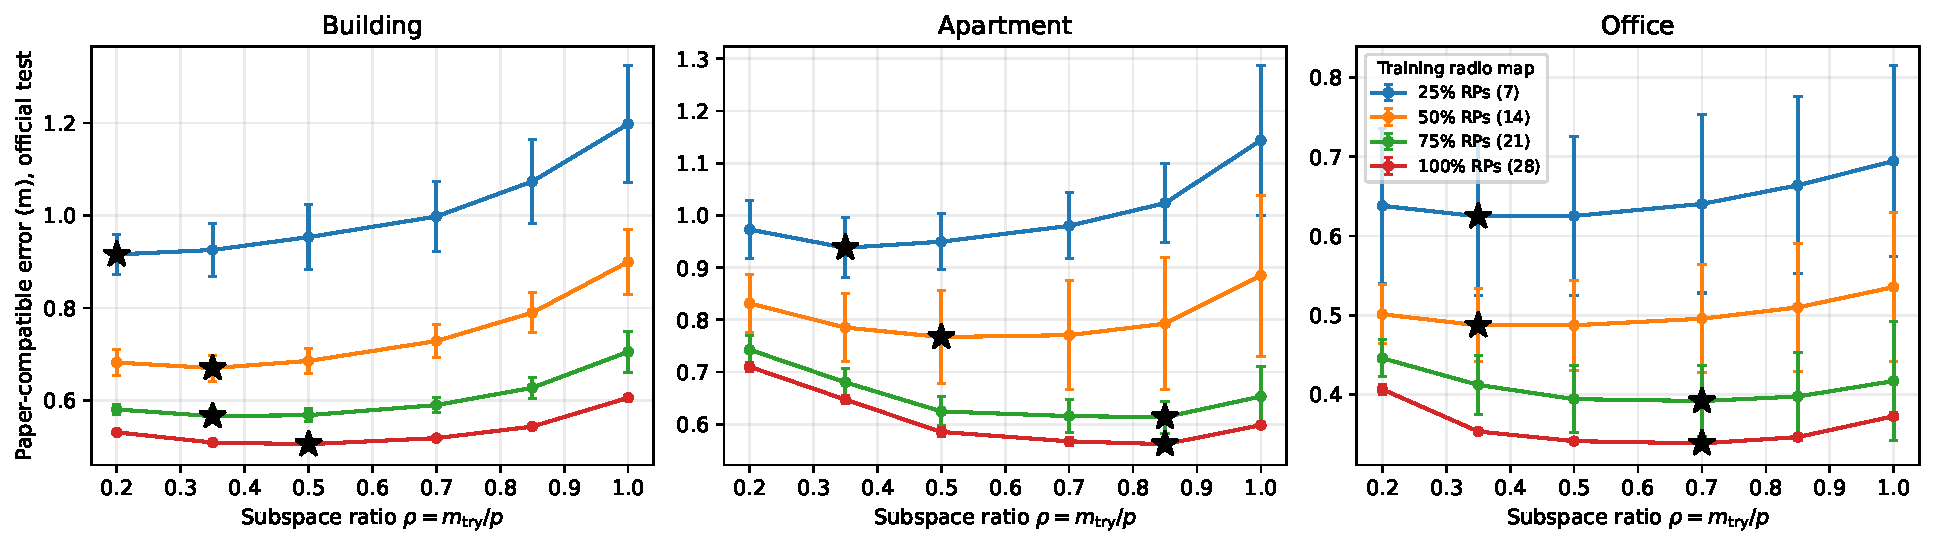
\includegraphics[width=\textwidth]{figures/results/fig13_density_ratio.pdf}
	\caption{Official-test error versus subspace ratio for training radio maps thinned to $100\%$, $75\%$, $50\%$, and $25\%$ of their RPs (number of RPs in parentheses; mean $\pm$ standard deviation over ten random RP subsets). Stars mark the best ratio of each curve.}
	\label{fig:density_ratio}
\end{figure*}

Three observations hold. First, $\rho=1$ is never the best ratio. In Building it is the worst ratio at every density, and in Apartment and Office it is the worst at $50\%$ and $25\%$. Second, the best ratio decreases as the map becomes sparser in all three environments (Table~\ref{tab:density_rf_et}):
\begin{itemize}
	\item Building: from $0.5$ at full density to $0.35$ at $75\%$ and $50\%$, and $0.2$ at $25\%$;
	\item Apartment: from $0.85$ at $100\%$ and $75\%$ (where $0.7$ is within $0.005$~m) to $0.5$ at $50\%$ and $0.35$ at $25\%$;
	\item Office: from $0.7$ at $100\%$ and $75\%$ to $0.35$ at $50\%$ and $25\%$.
\end{itemize}
Third, the gain of the best ratio over bagging tends to increase with sparsity. It rises from $16.6\%$ (full) to $25.5\%$ ($50\%$) in Building and from $6.1\%$ to $18.0\%$ ($25\%$) in Apartment. In Office, with only 28 training RPs (7 at $25\%$), it stays between $6\%$ and $10\%$. The fixed default $\rho=0.7$ improves on $\rho=1$ at every density ($5.2$--$19.0\%$), but on the sparsest maps it leaves part of the attainable gain unused (e.g., $0.998$ versus $0.916$~m in Building at $25\%$).

These results are consistent with per-split randomization acting as regularization~\cite{mentch2020randomization}: predicting positions between sparsely surveyed RPs is a noisier interpolation problem, for which stronger randomization is preferable. To test whether the effect is specific to Random Forests, the same thinned maps were used to train extremely randomized trees~\cite{geurts2006extremely} with the same ratio grid (Table~\ref{tab:density_rf_et}).

\begin{table*}[!t]
\centering
\caption{Density dependence of the optimal subspace ratio for Random Forests and extremely randomized trees (official test, paper-compatible metric, mean over 10 random RP subsets; both models use the same thinned radio maps). Best $\rho$: ratio with the lowest mean error in $\{0.2,0.35,0.5,0.7,0.85,1.0\}$. Gain: reduction of the best ratio relative to $\rho=1$.}
\label{tab:density_rf_et}
\footnotesize
\setlength{\tabcolsep}{4pt}
\begin{tabular}{llcccccc}
\toprule
 & & \multicolumn{3}{c}{Random Forest} & \multicolumn{3}{c}{Extremely randomized trees} \\
\cmidrule(lr){3-5}\cmidrule(lr){6-8}
Dataset & Training map & Best $\rho$ & Error (m) & Gain (\%) & Best $\rho$ & Error (m) & Gain (\%) \\
\midrule
Building & 100\% (483) & 0.50 & 0.505 & 16.6 & 1.00 & 0.545 & 0.0 \\
 & 75\% (362) & 0.35 & 0.566 & 19.8 & 1.00 & 0.594 & 0.0 \\
 & 50\% (242) & 0.35 & 0.670 & 25.5 & 1.00 & 0.696 & 0.0 \\
 & 25\% (121) & 0.20 & 0.916 & 23.6 & 0.50 & 0.971 & 0.4 \\
\midrule
Apartment & 100\% (81) & 0.85 & 0.562 & 6.1 & 1.00 & 0.617 & 0.0 \\
 & 75\% (61) & 0.85 & 0.613 & 6.1 & 1.00 & 0.659 & 0.0 \\
 & 50\% (40) & 0.50 & 0.767 & 13.3 & 1.00 & 0.757 & 0.0 \\
 & 25\% (20) & 0.35 & 0.938 & 18.0 & 1.00 & 0.903 & 0.0 \\
\midrule
Office & 100\% (28) & 0.70 & 0.338 & 9.2 & 1.00 & 0.349 & 0.0 \\
 & 75\% (21) & 0.70 & 0.392 & 6.1 & 1.00 & 0.392 & 0.0 \\
 & 50\% (14) & 0.35 & 0.487 & 9.0 & 0.50 & 0.443 & 0.8 \\
 & 25\% (7) & 0.35 & 0.625 & 10.1 & 1.00 & 0.583 & 0.0 \\
\bottomrule
\end{tabular}
\end{table*}


For extremely randomized trees, the best ratio is $\rho=1$ at almost every density, and feature subsampling never improves the error by more than $0.8\%$. The density dependence is therefore specific to Random Forests. This is consistent with the regularization interpretation: extremely randomized trees already draw their split thresholds at random, which provides strong randomization, so additional feature subsampling has nothing left to regularize. The comparison also shows that the two ensembles are complementary rather than interchangeable: with the best ratio, RF is more accurate in Building at every density, whereas extremely randomized trees are more accurate on the $50\%$ and $25\%$ Apartment and Office maps.

% ============================================================
\subsection{Choosing the Subspace Ratio}
\label{subsec:selection_results}

If the best ratio depends on density, it matters which data are used to choose it. Table~\ref{tab:ratio_selection} reports the test regret of each selection rule; the corresponding error curves are shown in Fig.~S8 of the supplementary material.

\begin{table*}[!t]
\centering
\caption{Selecting the subspace ratio. For each rule, the selected $\rho$ and the resulting regret on the official RP-disjoint test set (percentage above the best ratio of the sweep, $\rho\in\{0.2,0.35,0.5,0.7,0.85,1.0\}$, paper-compatible metric, seed 0). The test set is used only to score the rules, never to select $\rho$.}
\label{tab:ratio_selection}
\footnotesize
\setlength{\tabcolsep}{4pt}
\begin{tabular}{lccccccc}
\toprule
 & \multicolumn{2}{c}{Building} & \multicolumn{2}{c}{Apartment} & \multicolumn{2}{c}{Office} & \\
\cmidrule(lr){2-3}\cmidrule(lr){4-5}\cmidrule(lr){6-7}
Selection rule & $\rho$ & Regret (\%) & $\rho$ & Regret (\%) & $\rho$ & Regret (\%) & Worst (\%) \\
\midrule
Out-of-bag error (sample level) & 0.35 & 1.0 & 0.50 & 1.9 & 0.35 & 6.0 & 6.0 \\
5-fold sample-level CV & 0.35 & 1.0 & 0.50 & 1.9 & 0.35 & 6.0 & 6.0 \\
5-fold RP-grouped CV & 0.35 & 1.0 & 0.50 & 1.9 & 0.20 & 22.5 & 22.5 \\
Leave-one-environment-out minimax (RP-grouped CV) & 0.35 & 1.0 & 0.35 & 12.5 & 0.35 & 6.0 & 12.5 \\
Fixed $\rho=1.0$ (bagging; Feng et al.) & 1.00 & 19.7 & 1.00 & 6.4 & 1.00 & 12.1 & 19.7 \\
Fixed $\rho=0.7$ (this work) & 0.70 & 4.1 & 0.70 & 0.0 & 0.70 & 0.6 & 4.1 \\
Fixed $\rho=0.5$ & 0.50 & 0.0 & 0.50 & 1.9 & 0.50 & 0.0 & 1.9 \\
Fixed $\rho=0.35\approx1/3$ (Breiman) & 0.35 & 1.0 & 0.35 & 12.5 & 0.35 & 6.0 & 12.5 \\
\bottomrule
\end{tabular}
\end{table*}


The OOB error is between $0.04$ and $0.25$~m, an order of magnitude below the test error, because every scan is predicted by trees trained on other scans of the same RP; sample-level CV behaves the same way. Both estimators, and RP-grouped CV, select ratios of $0.2$--$0.5$, smaller than the test optimum ($0.5$--$0.7$). For RP-grouped CV this is the density effect of Section~\ref{subsec:density_results}: its fold models see a sparser map. As a result, the data-driven rules incur worst-case test regrets of $6.0$--$22.5\%$ (the leave-one-environment-out rule $12.5\%$) and bagging $19.7\%$, whereas the fixed default $\rho=0.7$ stays within $4.1\%$ of the best ratio in every environment and $\rho=0.5$ within $1.9\%$. The test curves are flat between $0.5$ and $0.7$, so for fully surveyed maps any ratio in this range is a robust default, while sparser maps favor smaller ratios.

The EETAC sweep (three seeds) is consistent with this picture. EETAC has only 25 RPs, i.e., a sparse map by the standards of Fig.~\ref{fig:density_ratio}, and its within-day sample-level and RP-grouped protocols are best at $\rho=0.35$--$0.5$. Across days, very small ratios become harmful in the seven-AP scenario (2D RMSE $3.19$~m at $\rho=0.2$ for Day~1$\rightarrow$Day~2), presumably because trees are then forced to split on Linksys APs whose measurements change between days, and the best cross-day ratios are $0.5$--$0.85$. In every EETAC protocol and scenario, $\rho=0.7$ is better than $\rho=1$.

% ============================================================
\subsection{Comparison with Literature Ensembles}
\label{subsec:literature_results}

The previous analyses vary only the subspace ratio of one RF. Table~\ref{tab:literature_baselines} places the configuration among other ensembles and a classical fingerprinting baseline: Breiman's default $m_{\mathrm{try}}=\lfloor p/3\rfloor$, extremely randomized trees, Rotation Forest, gradient-boosted trees, and WKNN.

\begin{table*}[!t]
\centering
\caption{Comparison with tree-ensemble and fingerprinting alternatives from the literature (paper-compatible metric, m). Test: official RP-disjoint test set. CV: pooled 5-fold RP-grouped CV on the training RPs. Office and Apartment: mean of three seeds; Building: one seed. Best value per column in bold.}
\label{tab:literature_baselines}
\footnotesize
\setlength{\tabcolsep}{4pt}
\begin{tabular}{lcccccc}
\toprule
 & \multicolumn{2}{c}{Building} & \multicolumn{2}{c}{Apartment} & \multicolumn{2}{c}{Office} \\
\cmidrule(lr){2-3}\cmidrule(lr){4-5}\cmidrule(lr){6-7}
Model & Test & CV & Test & CV & Test & CV \\
\midrule
RF, $\rho=1.0$ (bagging) \cite{feng2026robust} & 0.605 & 0.887 & 0.598 & 0.705 & 0.373 & 0.602 \\
RF, $\rho=0.7$ (this work) & 0.526 & 0.707 & \textbf{0.564} & 0.617 & \textbf{0.339} & 0.464 \\
RF, $m_{\mathrm{try}}=\lfloor p/3\rfloor$ \cite{breiman2001random} & \textbf{0.515} & \textbf{0.649} & 0.640 & 0.621 & 0.351 & 0.424 \\
Extremely randomized trees \cite{geurts2006extremely} & 0.543 & 0.698 & 0.616 & \textbf{0.611} & 0.346 & \textbf{0.386} \\
Rotation Forest \cite{rodriguez2006rotation} & 0.520 & 0.652 & 0.704 & 0.619 & 0.386 & 0.394 \\
Gradient-boosted trees (500 iterations) & 0.620 & 0.765 & 0.834 & 0.683 & 0.352 & 0.431 \\
WKNN, $k=5$ \cite{bahl2000radar} & 0.941 & 1.139 & 0.853 & 0.842 & 0.401 & 0.465 \\
\bottomrule
\end{tabular}
\end{table*}


No method is best everywhere. On the official test sets, RF300-F0.7 is best in Office and Apartment and within $0.011$~m of the best model (RF with $\lfloor p/3\rfloor$) in Building. Under RP-grouped CV, i.e., on sparser maps, the more strongly randomized ensembles lead: extremely randomized trees in Office and Apartment, and RF with $\lfloor p/3\rfloor$ and Rotation Forest in Building. This ordering again matches the density effect. Gradient-boosted trees, a strong general-purpose tabular baseline, are less accurate than RF300-F0.7 on every official test set (e.g., $0.620$ versus $0.526$~m in Building and $0.834$ versus $0.564$~m in Apartment). WKNN, the classical fingerprinting baseline, is clearly worse in the two larger environments. All bagging-based randomized ensembles improve on the full-feature RF used in prior work.

% ============================================================
\subsection{Accuracy--Efficiency Trade-off}
\label{subsec:efficiency_results}

Accuracy is only one side of the comparison. The measured cost of the two 300-tree models is reported in the supplementary material (Table~S7). Wall-clock training and inference times vary with the environment and system load; for example, Building training took $13.63$~s for RF300-F1.0 and $6.35$~s for RF300-F0.7 in this run, with inference times of $12.93$ and $9.29~\mu$s per scan. At equal tree count, the subsampled model is $9$--$19\%$ larger in serialized size, because its trees are deeper.

Fig.~\ref{fig:model_size} (values in Table~S11 of the supplementary material) shows that the accuracy gained by subsampling can be traded for model size. A 100-tree RF0.7 forest matches or slightly improves on the 300-tree RF0.7 forest in all three environments; a 50-tree forest loses $0.004$--$0.010$~m. In Building, the 50-tree RF0.7 forest is $10.7$~MB instead of $58.8$~MB for the 300-tree full-feature model ($5.5\times$ smaller), infers in about $2~\mu$s per scan on one thread instead of about $13~\mu$s, and is still $11.4\%$ more accurate ($0.536$ versus $0.605$~m). The corresponding Office and Apartment models occupy $0.56$ and $2.49$~MB. The compact Building model remains larger than the 93,934-parameter GTCN~\cite{rana2025gtcn}, which reports a lower 2D RMSE ($0.660$~m) at the cost of roughly 38~min of training.

\begin{figure*}[!t]
	\centering
	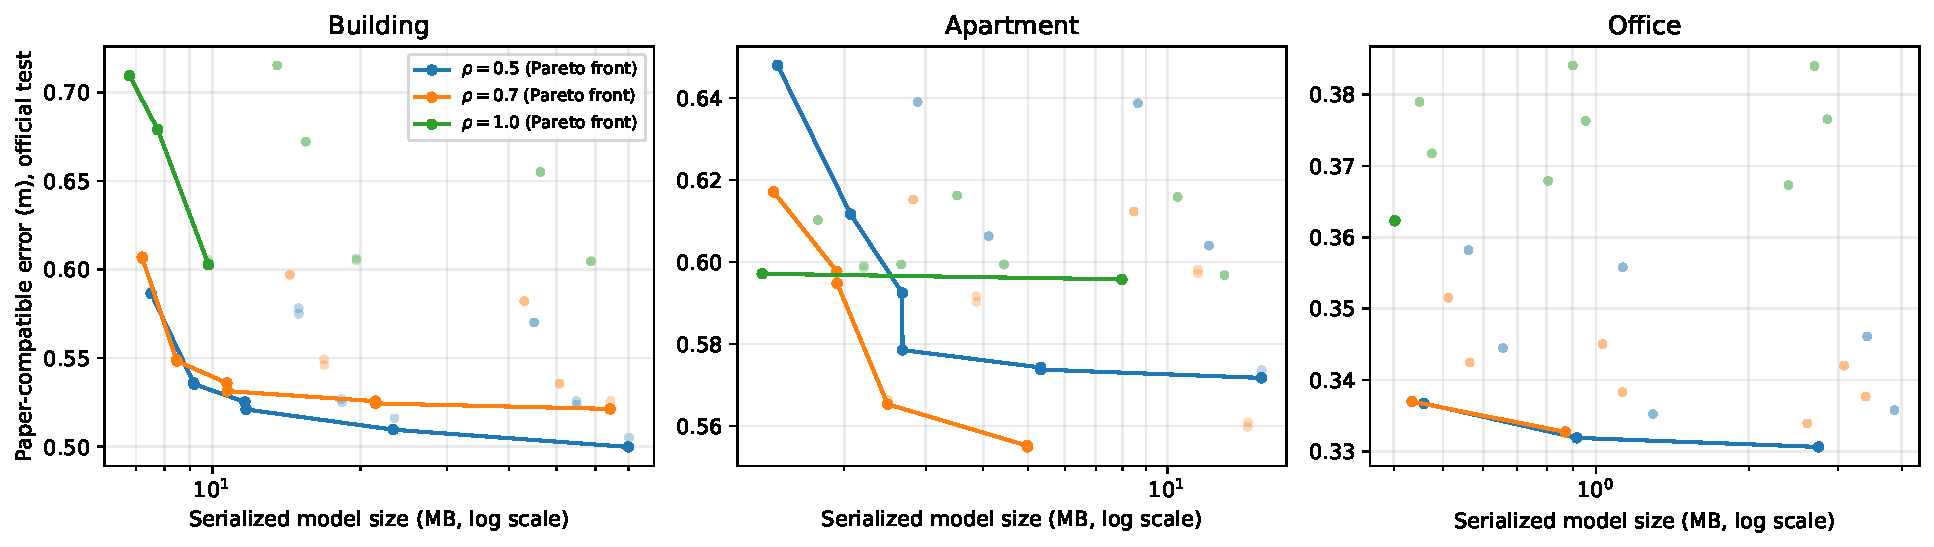
\includegraphics[width=\textwidth]{figures/results/fig15_model_size.pdf}
	\caption{Official-test error versus serialized model size for forests with 50--300 trees, minimum leaf sizes 1--20, and depth limits, for $\rho\in\{0.5,0.7,1.0\}$. Lines show the Pareto front of each ratio.}
	\label{fig:model_size}
\end{figure*}

% ============================================================
\subsection{Uncertainty-Region Performance}
\label{subsec:uncertainty_results}

We finally turn from point accuracy to uncertainty regions. Table~\ref{tab:calibration_rules} compares the three calibration rules of Section~\ref{subsec:strict_conformal} over repeated random RP-level fit/calibration splits. Since the guarantee of split conformal prediction concerns the coverage averaged over calibration draws, the mean coverage is the relevant criterion for validity; the minimum shows how much a single deployment can deviate from it. Reserving calibration RPs has a cost for the point predictor: trained on the $\sim$75\% fitting subset instead of all training RPs, RF300-F0.7 is $13.6\%$ less accurate in Building and $11.7\%$ in Apartment, and essentially unchanged in Office (Table~S10 of the supplementary material).

\begin{table*}[!t]
\centering
\caption{Split-conformal calibration of circular regions when the $\sim$120 scans of each RP are correlated, over repeated random RP-level fit/calibration splits ($25\%$ of training RPs for calibration; coverage on the official test set). Scan-level: all calibration scans treated as exchangeable. Group: one randomly chosen scan per calibration RP, with ordinary split conformal on these $G$ scores, which is valid when RPs are exchangeable~\cite{Dunn02102023}. RP-count: pooled scores with the finite-sample level computed from $G$. The guarantee of a valid method concerns the mean coverage over calibration draws; individual splits vary around it.}
\label{tab:calibration_rules}
\footnotesize
\setlength{\tabcolsep}{4pt}
\begin{tabular}{llcccccc}
\toprule
 & & \multicolumn{3}{c}{$1-\alpha=0.90$} & \multicolumn{3}{c}{$1-\alpha=0.95$} \\
\cmidrule(lr){3-5}\cmidrule(lr){6-8}
Dataset & Calibration rule & Mean cov. & Min cov. & Area (m$^2$) & Mean cov. & Min cov. & Area (m$^2$) \\
\midrule
Building ($G=121$, 10 splits) & Scan-level (standard) & 0.940 & 0.917 & 5.98 & 0.974 & 0.962 & 9.80 \\
 & Group, one scan per RP (valid) & 0.946 & 0.913 & 6.55 & 0.978 & 0.959 & 11.45 \\
 & RP-count (conservative heuristic) & 0.946 & 0.924 & 6.31 & 0.978 & 0.965 & 10.97 \\
\midrule
Apartment ($G=21$, 20 splits) & Scan-level (standard) & 0.894 & 0.838 & 6.63 & 0.931 & 0.895 & 9.12 \\
 & Group, one scan per RP (valid) & 0.916 & 0.871 & 8.10 & 0.947 & 0.897 & 11.88 \\
 & RP-count (conservative heuristic) & 0.932 & 0.896 & 9.25 & 0.995 & 0.968 & 33.19 \\
\midrule
Office ($G=7$, 20 splits) & Scan-level (standard) & 0.947 & 0.809 & 4.09 & 0.958 & 0.853 & 5.02 \\
 & Group, one scan per RP (valid) & \multicolumn{3}{c}{no finite region ($G<1/\alpha-1$)} & \multicolumn{3}{c}{no finite region ($G<1/\alpha-1$)} \\
 & RP-count (conservative heuristic) & 0.980 & 0.898 & 8.88 & 0.980 & 0.898 & 8.88 \\
\bottomrule
\end{tabular}
\end{table*}


With 121 calibration RPs (Building), the three rules agree: all over-cover moderately ($0.94$--$0.98$), and the group and RP-count regions are $5$--$17\%$ larger than the scan-level ones. With $G=21$ (Apartment), the scan-level rule falls below the nominal level on average ($0.894$ at $90\%$, $0.931$ at $95\%$) and under-covers in $65\%$ and $75\%$ of the splits. The group rule, which uses one scan per RP and is valid when RPs are exchangeable~\cite{Dunn02102023}, restores the nominal mean coverage ($0.916$ and $0.947$) with regions $22$--$30\%$ larger. Individual splits still fall below the nominal level, as expected for a marginal guarantee with only 21 calibration scores. The RP-count correction over-covers ($0.932$ and $0.995$); at $95\%$, where $G<2/\alpha-1$, its threshold is the largest pooled score and the region grows to $33.2$~m$^2$, nearly three times the group region.

With $G=7$ (Office), the group rule has no finite region at either level, because $G<1/\alpha-1$. The scan-level rule gives finite regions but under-covers in $25$--$35\%$ of the splits (minimum $0.809$), and the RP-count heuristic has no guarantee. Seven calibration RPs are therefore too few for a valid circle at these levels. In general, a valid group calibration needs at least $1/\alpha-1$ held-out RPs (9 at $90\%$, 19 at $95\%$), and its region shrinks toward the scan-level region as $G$ grows. This gives a direct survey-planning rule for uncertainty-aware fingerprinting.

The single-split results in the supplementary material (Table~S8) compare circles with covariance-aware ellipses. With scan-level calibration, the ellipse is $3.7$--$7.8\%$ smaller than the circle under split conformal and $6.0$--$13.0\%$ smaller under grouped OOF. Its coverage is close to that of the circle in Building but lower in Office and Apartment, so the ellipse is a more compact anisotropic description of the error, not a better-calibrated region.

% ============================================================
\subsection{Summary of Main Findings}
\label{subsec:results_summary}

The main findings of this section are:

\begin{itemize}
	\item Full-feature bagging is never the best ratio; RF300-F0.7 reduces the reproduced baseline error by $14.3\%$, $7.1\%$, and $5.1\%$ on the official tests (significant for Building and Office; lower error in all ten seeds in every environment) and by $20.1\%$, $22.1\%$, and $12.2\%$ under RP-grouped CV.
	\item For Random Forests, the optimal ratio decreases as the radio map becomes sparser in all three environments, and the gain over bagging reaches $25.5\%$; extremely randomized trees gain at most $0.8\%$ from subsampling. The fixed default $\rho=0.7$ is within $4.1\%$ of the best ratio at full density, whereas OOB, sample-level, and RP-grouped selection are biased toward small ratios.
	\item On the frame-aligned EETAC dataset, RF300-F0.7 improves 2D RMSE by $11$--$14\%$ in sample-level and RP-grouped CV and is better in 74 of 80 seed--protocol comparisons; one cross-day direction (High, Day~1$\rightarrow$Day~2) is a tie.
	\item No literature ensemble is best everywhere; the strongest one depends on map density, randomized bagging ensembles all improve on the full-feature RF, and gradient boosting and WKNN are less accurate.
	\item 50--100-tree subsampled forests are more accurate than the 300-tree full-feature forest while being $2.5$--$5.5$ times smaller.
	\item With 21 calibration RPs, scan-level conformal calibration falls below the nominal coverage on average, whereas group calibration with one scan per RP attains it with $22$--$30\%$ larger regions; with 7 RPs no valid finite region exists, and the RP-count heuristic is conservative.
\end{itemize}
